\documentclass[11pt]{article}
\usepackage[margin=1in]{geometry}
% \usepackage[preprint]{neurips_2024}
\usepackage{graphicx}
\usepackage{amsmath}
\usepackage{amssymb}
\usepackage{hyperref}
\usepackage{cite}
\usepackage{titlesec}
\usepackage{float}
\usepackage{adjustbox} 
\usepackage{listings}
\usepackage{xcolor}
\usepackage{multicol}
\setcounter{secnumdepth}{4}

\title{PlantPal - helping you be a better \textit{pal} to your plants
}
\author{
    \begin{tabular}[t]{l}
        SNEHA SARKAR \\
        \texttt{A0304787U} \\
        \texttt{e1373875@u.nus.edu} \\
    \end{tabular}
    \and
    \begin{tabular}[t]{l}
        MANAV KAMLESH CHOUHAN \\
        \texttt{A0304485A} \\
        \texttt{e1373573@u.nus.edu} \\
    \end{tabular}
    \and
    \begin{tabular}[t]{l}
        SHEN AO \\
        \texttt{A0297059M} \\
        \texttt{e1351197@u.nus.edu} \\
    \end{tabular}
    \and
    \begin{tabular}[t]{l}
        TEO XUAN WEI \\
        \texttt{A0168645R} \\
        \texttt{e0177078@u.nus.edu} \\
    \end{tabular}
    \and
    \begin{tabular}[t]{l}
        BHUSHAN GANESH MOHOL \\
        \texttt{A0304884X} \\
        \texttt{e1373972@u.nus.edu}
    \end{tabular}
}

\begin{document}

\maketitle

\section{Theme}
Singapore is well known for its City in a Garden vision, where greenery is integrated into urban living. With the nation’s focus on sustainability, food security, and community well-being, there is growing interest in urban farming, ornamental plant ownership, and smart agricultural solutions. PlantPal fits into this landscape by offering an accessible digital tool for plant disease detection and care recommendations, supporting both national goals and individual needs.

\begin{enumerate}
    \item Urban Farming \& Community Gardens: Singapore has actively promoted urban farming and community gardening through NParks’ \textit{Community in Bloom} programme. Residents often cultivate herbs, orchids, and vegetables in HDB void decks, balconies, and rooftop gardens. PlantPal can support these efforts by enabling gardeners to quickly diagnose plant diseases, ensuring healthier crops in limited urban spaces.

    \item Smart Nation \& Sustainability Goals: Aligned with the \textit{30 by 30} vision to produce 30\% of Singapore’s nutritional needs locally by 2030, local farms and nurseries face ongoing pest and disease challenges. PlantPal offers a low-cost, scalable way to detect plant diseases early and recommend interventions, helping reduce crop losses and contributing to national food security.

    \item Relevance for Hobbyists \& Collectors: Beyond urban farming, plant ownership is a widespread hobby in Singapore. Ornamental plants such as orchids, succulents, and rare tropical foliage (e.g., monstera, philodendrons) are highly prized, with some rare orchids valued at hundreds of dollars. PlantPal helps hobbyists protect these valuable plants by identifying early signs of disease, safeguarding both their collections and investments.
\end{enumerate}


\section{Business Model}

PlantPal will operate on a freemium model tailored to different user groups, ensuring accessibility for hobbyists while generating sustainable revenue from farms and enterprises.

\begin{enumerate}
    \item Hobbyists \& Home Gardeners (B2C):
    \begin{itemize}
        \item Free Tier:
        \begin{itemize}
            \item Upload plant images for basic disease detection.
            \item 
        Receive general care tips and treatment suggestions.
        \end{itemize}
        \item Premium Tier (Subscription / Pay-per-use):
        \begin{itemize}
            \item Detailed diagnostic reports (disease probability, severity).
            \item Personalized plant care recommendations.
            \item Plant health tracking over time.
            \item Estimated: SGD 3–5/month or SGD 1 per premium scan.
        \end{itemize}
    \end{itemize}
    \item Community Gardens \& Small Farms (B2B Lite)
    \begin{itemize}
        \item Affordable subscription plan for groups or small farms.
        \item Features:
        \begin{itemize}
            \item Bulk scanning (multiple images per day).
            \item Data dashboard to monitor crop health trends.
            \item Seasonal advice for pest/disease prevention.
            \item Estimate: SGD 30–50/month.
        \end{itemize}
    \end{itemize}
    \item Commercial Farms \& Nurseries (B2B Enterprise)
    \begin{itemize}
        \item Tailored enterprise solution with:
        \begin{itemize}
            \item API access for integration into farm management systems.
            \item Advanced analytics on crop disease trends.
            \item Multi-user access and priority support.
            \item Pricing via custom contracts.
        \end{itemize}
    \end{itemize}
    \item Add-on Revenue Streams:
    \begin{itemize}
        \item Plant Care Marketplace: Partner with nurseries, garden shops, and agri-tech suppliers to suggest remedies (fertilizers, pesticides, soil care products) within the app. Earn referral fees or commission on sales.
        \item Data Insights: Aggregated, anonymized plant health data could support urban farming research or government food security initiatives.
    \end{itemize}
\end{enumerate}

\section{Cloud service}

PlantPal will be deployed as a cloud-native service on AWS to ensure scalability, reliability, and accessibility for both individual users and enterprise partners. The system integrates a FastAPI backend with cloud storage, machine learning (ML) inference, and a React-based frontend.

\begin{enumerate}
    \item Core Functionality
    \begin{itemize}
        \item Plant Disease Detection API (FastAPI)
        \begin{itemize}
            \item Users upload plant images through the web interface.
            \item Images are sent to the FastAPI backend (containerized and deployed on AWS ECS or EKS).
            \item Backend triggers ML inference (plant species classification + disease detection).
            \item Output: prediction with confidence scores.
        \end{itemize}

        \item Recommendation Engine (FastAPI)
        \begin{itemize}
            \item Backend retrieves care instructions based on detected disease/species.
            \item  Advice includes watering schedules, pruning, and treatment suggestions.
        \end{itemize}

        \item User Engagement Features
        \begin{itemize}
            \item Health tracking dashboards.
            \item Notifications/reminders (via email or mobile push).
            \item Gamification (badges, streaks, milestones).
        \end{itemize}
\end{itemize}

\item Benefits of Cloud Deployment:
\begin{itemize}
    \item Scalability: ECS can auto-scale FastAPI containers during peak demand.
    \item Security: IAM roles + S3 bucket policies restrict access.
    \item Reliability: CloudFront ensures low-latency global delivery.
    \item Cost-Efficiency: Pay-per-use compute/storage; lightweight architecture for hobbyist use cases.
\end{itemize}

\end{enumerate}

\section{Preliminary design}

\begin{itemize}
    \item Frontend:
    \begin{itemize}
        \item React.js application with Tailwind CSS for responsive UI design.
        \item Static assets hosted on Amazon S3 with global delivery via CloudFront CDN.
    \end{itemize}
    \item Backend API Layer:
    \begin{itemize}
        \item FastAPI containerized application deployed on AWS ECS with EC2 launch type.
        \item RESTful API endpoints for plant scanning, user management, and care recommendations.
        \item Asynchronous processing for ML inference and external API calls.
        \item JWT token validation for secure authenticated requests
        \item SQL Alchemy as ORM with Alembic for database migration and change management.
    \end{itemize}
    \item Database Layer:
    \begin{itemize}
        \item SQL database hosted on Amazon RDS (PostgreSQL Engine).
        \item Stores user profiles, plant records, scan history, gamification records and personalized recommendations.
    \end{itemize}
    \item CI/CD Pipeline:
    \begin{itemize}
        \item GitHub Actions workflows for automated build, test, and deployment.
        \item Frontend: React build → deploy to S3 → CloudFront cache invalidation.
        \item Backend: Docker build → push to ECR → ECS service update (blue-green deployments).
    \end{itemize}
    \item Machine Learning Integration:
    \begin{itemize}
        \item Amazon SageMaker endpoints for pretrained Hugging face disease detection, Plant Species Identification and custom care recommendation models.
    \end{itemize}
\end{itemize}
\begin{itemize}
    \item Virtual Private Cloud (VPC) Configuration:
    \begin{itemize}
        \item Application Load Balancer (ALB) in public subnet for traffic distribution.
        \item ECS tasks deployed in private subnets for enhanced security.
    \end{itemize}

    \item Security Implementation:
    \begin{itemize}
        \item AWS Cognito User Pools for centralized user authentication and management.
        \item Custom Lambda function for personalized email notifications (signup/password reset).
        \item IAM roles and policies for fine-grained service-to-service authentication.
        \item HTTPS/TLS encryption for all client-server communications.
        \item VPC Endpoints for secure access to S3, ECR, and CloudWatch services.
    \end{itemize}
\end{itemize}
\begin{figure}[H]
    \centering
    \href{https://drive.google.com/file/d/1lJucSu2xudmuGDQbB22ojH6RFfhKNEwI/view?usp=sharing}{
        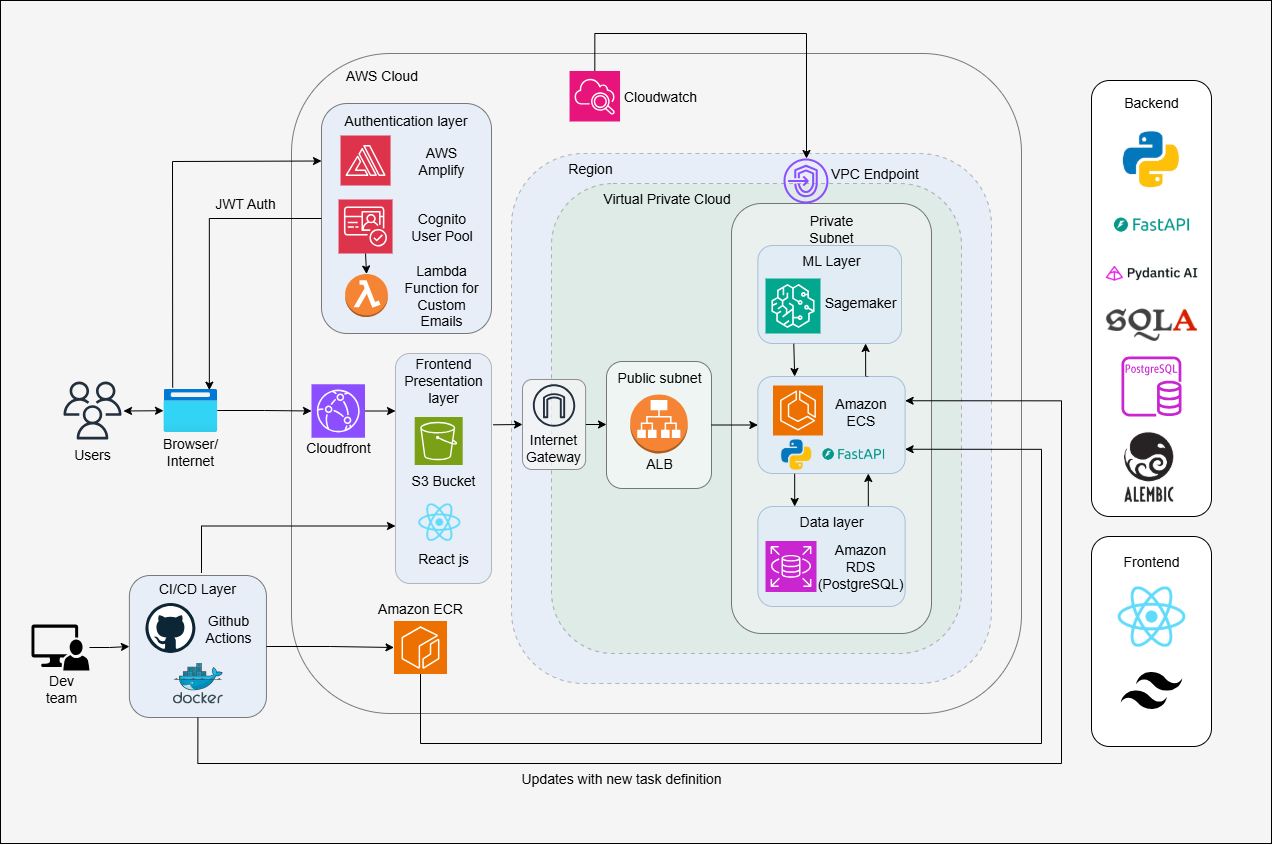
\includegraphics[width=1\linewidth]{Architecture.png}
    }
    \caption{System Architecture}
    \label{fig:System Architecture}
\end{figure}

\section{Implementation plan}
\subsection*{Phase 1: Requirements, Design \& Setup (Week 1)}
\begin{itemize}
    \item Finalize functional and non-functional requirements.
    \item Design and refine the system architecture.
    \item Set up AWS accounts, GitHub repository, and CI/CD skeleton.
\end{itemize}

\subsection*{Phase 2A: Frontend Development (Weeks 2–4)}
\begin{itemize}
    \item Build React frontend and core UI components (upload photo, login/signup, dashboard, streaks).
    \item Implement user authentication flows (signup, login, password reset) with Cognito and personalized email templates via Lambda.  
    \item Setup mock backend responses.
    \item Connect Cognito JWT validation.
\end{itemize}

\subsection*{Phase 2B: Backend Development \& Database (Weeks 2-4)}
\begin{itemize}
    \item Set up FastAPI backend in ECS via ECR, with necessary IAM Roles.
    \item Implement REST endpoints for user management, plant scan submission, care recommendations and gamification logic.
    \item Configure PostgreSQL on RDS; apply initial migrations.
\end{itemize}

\subsection*{Phase 3: ML Integration (Weeks 5-6)}
\begin{itemize}
    \item Deploy Plant and Disease Detection model endpoint on SageMaker / HuggingFace / EC2.
    \item Deploy LLM recommendation model endpoint on SageMaker HuggingFace / EC2.
    \item Develop error handling and fallback logic.
    \item Connect with backend and frontend.
\end{itemize}

\subsection*{Phase 4: CI/CD \& Quality Assurance (Week 7)}
\begin{itemize}
    \item Finalize GitHub Actions workflows for frontend and backend. 
    \item Monitor via CloudWatch (spans all weeeks).
    \item Add automated tests: unit tests for backend, integration tests for API, and basic UI tests.  
\end{itemize}

\subsection*{Phase 5: Final Testing, Polishing \& Report
(Weeks 8-9)}
\begin{itemize}
    \item Conduct end-to-end testing: user signup, image upload, ML inference, and recommendation display.  
    \item Performance and security testing; optimize container and database configurations.
    \item Prepare project report.
\end{itemize}

\end{document}



 